\documentclass[a4paper, 12pt]{article}
\usepackage{cmap}
\usepackage{amssymb}
\usepackage{amsmath}
\usepackage{graphicx}
\usepackage{amsthm}
\usepackage{upgreek}
\usepackage{setspace}
\usepackage{color}
\usepackage{pgfplots}
\pgfplotsset{compat=1.9}
\usepackage[T2A]{fontenc}
\usepackage[utf8]{inputenc}
\usepackage[normalem]{ulem}
\usepackage{mathtext} % русские буквы в формулах
\usepackage[left=2cm,right=2cm, top=2cm,bottom=2cm,bindingoffset=0cm]{geometry}
\usepackage[english,russian]{babel}
\usepackage[unicode]{hyperref}
\newenvironment{Proof} % имя окружения
{\par\noindent{$\blacklozenge$}} % команды для \begin
{\hfill$\scriptstyle\boxtimes$}
\newcommand{\Rm}{\mathbb{R}}
\newcommand{\Cm}{\mathbb{C}}
\newcommand{\Z}{\mathbb{Z}}
\newcommand{\I}{\mathbb{I}}
\newcommand{\N}{\mathbb{N}}
\newcommand{\rank}{\operatorname{rank}}
\newcommand{\Ra}{\Rightarrow}
\newcommand{\ra}{\rightarrow}
\newcommand{\FI}{\Phi}
\newcommand{\Sp}{\text{Sp}}
\renewcommand{\leq}{\leqslant}
\renewcommand{\geq}{\geqslant}
\renewcommand{\alpha}{\upalpha}
\renewcommand{\beta}{\upbeta}
\renewcommand{\gamma}{\upgamma}
\renewcommand{\delta}{\updelta}
\renewcommand{\varphi}{\upvarphi}
\renewcommand{\phi}{\upvarphi}
\renewcommand{\tau}{\uptau}
\renewcommand{\lambda}{\uplambda}
\renewcommand{\psi}{\uppsi}
\renewcommand{\mu}{\upmu}
\renewcommand{\omega}{\upomega}
\renewcommand{\d}{\partial}
\renewcommand{\xi}{\upxi}
\renewcommand{\epsilon}{\upvarepsilon}
\newcommand{\intx}{\int\limits_{x_0}^x}
\newcommand\Norm[1]{\left\| #1 \right\|}
\newcommand{\sumk}{\sum\limits_{k=0}^\infty}
\newcommand{\sumi}{\sum\limits_{i=0}^\infty}
\newtheorem*{theorem}{Теорема}
\newtheorem*{cor}{Следствие}
\newtheorem*{lem}{Лемма}
\begin{document}
	\section*{Построение интерполяционного многочлена}
	\subsubsection*{Условие}
	Построить интерполяционный многочлен для функции $f(x) = 2^x$ по ее значениям в точках $x_0 = 0$, $x_1 = 2$, $x_2 = 3$. Вычислить с его помощью приближенное значение $f(0.5)$ и оценить погрешность найденного значения.
	\subsubsection*{Алгоритм решения}
	Для построения интерполяционного многочлена нам понадобятся следующие формулы:
	\begin{enumerate}
		\item формула Ньютона для интерполяционного многочлена \begin{multline}
			P_n(x) = f(x_0) + (x-x_0)\cdot f(x_0, x_1) + (x-x_0)(x-x_1)\cdot f(x_0,x_1,x_2) +\ldots \\ \ldots + (x-x_0)\ldots (x-x_{n-1})\cdot f(x_0,\ldots, x_n).
		\end{multline}
		\item аппарат разделенных разностей:
		\begin{itemize}
			\item \textbf{разделенная разность нулевого порядка для функции $f(x)$} совпадают со значениями функции $f(x_i)$ в узлах интерполирования;
			\item \textbf{разделенная разность первого порядка} есть \begin{eqnarray}
			f(x_i, x_j) = \dfrac{f(x_j) - f(x_i)}{x_j - x_i}.
			\end{eqnarray}
			\item \textbf{разделенная разность второго порядка} \begin{eqnarray}
			f(x_i, x_j, x_k) = \dfrac{f(x_j, x_k) - f(x_i, x_j)}{x_k - x_i}.
			\end{eqnarray}
			\item \textbf{разделенная разность $(k+1)$-ого порядка} \begin{eqnarray}
			f(x_0, \ldots, x_{k+1}) = \dfrac{f(x_1,\ldots, x_{k+1}) - f(x_0,\ldots, x_k)}{x_{k+1} - x_0}.
			\end{eqnarray}
		\end{itemize}
			 \item таблица разделенных разностей
			 	$$
			 	\includegraphics[scale=0.35]{"C:/Users/bzzdwn/Documents/Конспекты/Computational Methods/img9"}
			 	$$
			\item представление остатка интерполирования в форме Лагранжа
			\begin{eqnarray}
				r_n(x) = \omega_{n+1}(x) \dfrac{f^{(n+1)}(\xi)}{(n+1)!},\quad \xi \in [a,b].
			\end{eqnarray}
	\end{enumerate}
	Алгоритм решения задачи следующий: мы строим таблицу разделенных разностей, а затем, используя построенные разделенные разности, строим интерполяционный многочлен. После чего мы оцениваем остаток интерполирования, который и будет являться погрешностью в данном случае.\\\\
	Составляем таблицу разделенных разностей. Число столбцов таблицы = число узлов + 1. В нашем случае это 4:
	$$
		\includegraphics[scale=0.25]{"C:/Users/bzzdwn/Documents/Конспекты/Примеры ЧМ/img3"}
	$$
	Первый столбец заполняем значениями узлов, которые даны по условию. Для второго столбца вычислим значения функции в узлах:
	$$f(x_0) = 2^0 = 1,\quad f(x_1) = 2^2 = 4,\quad f(x_2) = 2^3 = 8.$$
	$$
		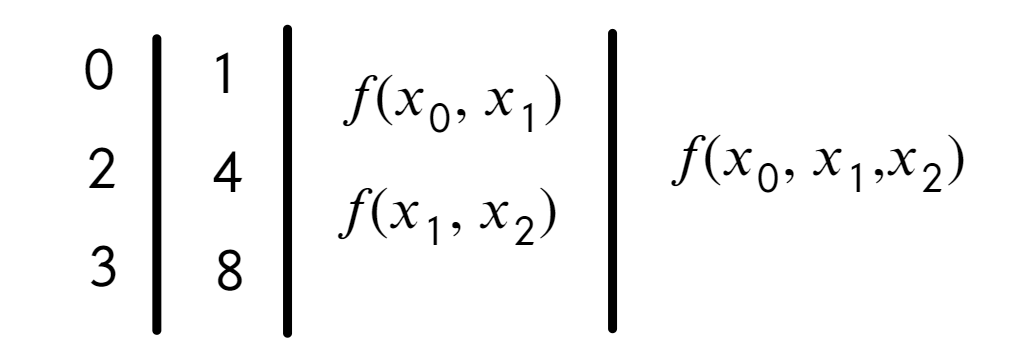
\includegraphics[scale=0.25]{img4}
	$$	
	По формуле (2) вычисляем значения для третьего столбца:
	$$f(x_0, x_1) = \dfrac{f(x_1) - f(x_0)}{x_1 - x_0} = \dfrac{4-1}{2-0} = \dfrac{3}{2},\quad f(x_1, x_2) = \dfrac{f(x_2) - f(x_1)}{x_2 - x_1} = \dfrac{8-4}{3-2} = 4.$$
	$$
		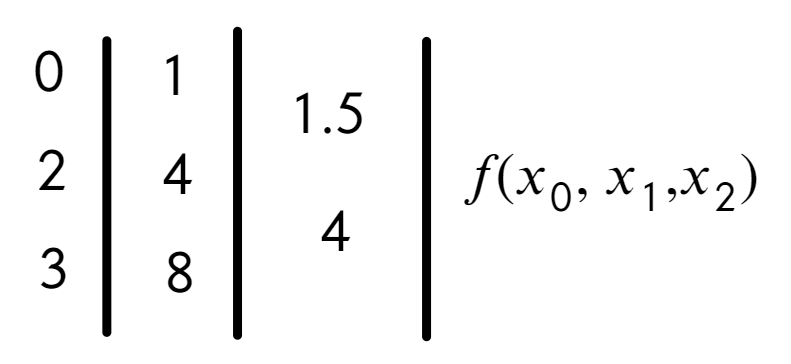
\includegraphics[scale=0.25]{img5}
	$$
	По формуле (3) вычисляем последнее неизвестное значение:
	$$f(x_0,x_1,x_2) = \dfrac{f(x_1, x_2) - f(x_0, x_1)}{x_2 - x_0} = \dfrac{4-1.5}{3-0} = \dfrac{5}{6}.$$
	Окончательно таблица имеет следующий вид, из которого нам понадобятся только выделенные значения:
	$$
		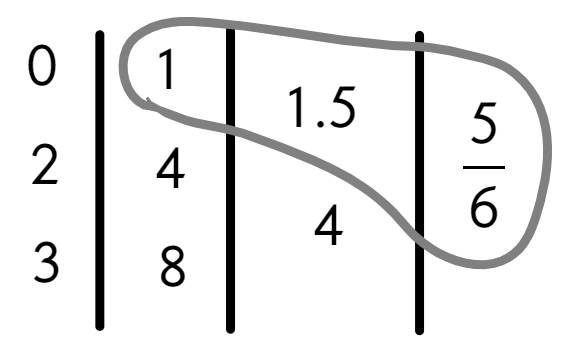
\includegraphics[scale=0.25]{img6}
	$$
	По формуле (1) строим интерполяционный многочлен, который в нашем случае имеет вид $$P_2(x) = f(x_0) + (x-x_0)\cdot f(x_0, x_1) + (x-x_0)(x-x_1)\cdot f(x_0,x_1,x_2).$$
	Подставляем все известные значения:
	$$P_2(x) = 1 + x\cdot \dfrac32 + x(x-2)\cdot \dfrac56 = \dfrac56x^2 - \dfrac16x + 1.$$
	Найдем значение в точке $x=0.5$:
	$$P_2(0.5) = \dfrac{5}{24} - \dfrac{1}{12} + 1 = \dfrac{27}{24}.$$
	Оценим остаток интерполирования, используя формулу (5):
	$$|r_n(x)| \leq \left|\omega_{n+1}(x) \dfrac{\underset{x\in[a,b]}{\max}|f^{(n+1)}(x)|}{(n+1)!}\right|.$$
	В нашем случае
	$$|r_2(x)| \leq \left|(x-x_0)(x-x_1)(x-x_2)| \dfrac{\underset{x\in[0,3]}{\max}|(2^x)^{(3)}(x)|}{3!}\right|.$$
	Так как $(2^^x)^{(n)} = \ln^n 2 2^x$, то $$\underset{x\in[0,3]}{\max}|2^x \cdot \ln^32|\leq (2\ln 2)^3.$$
	Тогда $$|r_2(x)|\leq \left|x(x-2)(x-3)\dfrac{(2\ln 2)^3}{6}\right|.$$
	Подставим точку, в которой мы проводили интерполирование, $x=0.5$:
	$$|r_2(0.5)|\leq \dfrac12\cdot \dfrac32\cdot\dfrac52\cdot\dfrac{(2\ln 2)^3}{6} = \dfrac52 \ln^32\approx 0.83256.$$
	Графически это можно представить как 
	\begin{center}\begin{tikzpicture}
		\begin{axis}[
			title = Function Interpolation,
			legend pos = north west,
			xlabel = {$x$},
			ylabel = {$y$},
			minor tick num = 2,
			xmin = -0.5,
			xmax = 3.5,
			grid = major,
			scatter/classes={%
				a={mark=o,draw=black}}
			]
			\legend{$2^x$, $P_2(x)$}
			\addplot[scatter,only marks,%
			scatter src=explicit symbolic]%
			table[meta=label] {
				x y label
				0 1 a
				2 4 a
				3 8 a
				};
			\addplot[orange] {5/6*x^2 - 1/6*x + 1};
		\end{axis}
		\end{tikzpicture}\end{center}
\end{document}